% Printed 488; principal PDF 495; Google PDF 499.
\par\clearpage
\noindent\makebox[0pt][l]{\fontsize{13}{16}\selectfont 488}\hfill{\small\textbf{NACHLASS.}}\hfill\null\par\medskip
\noindent paar dritten Ranges für die Erkundungen gebraucht. Die Messungen mit dem erstgenannten habe ich alle allein übernommen.

\par\noindent\hspace*{\parindent}Bei der neuen Aufgabe, die unmittelbarer die Geografie des Landes betrifft und bei der viele sekundäre und tertiäre Messungen vorgenommen werden müssen, werden daher auch mehrere Theodolite zweiten und dritten Ranges ständig gebraucht. Einen Theodoliten zweiten Ranges (den die Sternwarte seit 1813 besitzt) hat Herr Hauptmann \textsc{Müller} im vergangenen Sommer benutzt, eigentlich um damit seine ersten Übungen zu machen. Einen anderen (allerdings nicht ganz zufriedenstellenden) besitzt Herr Leutnant \textsc{Hartmann} selbst, der damit im vergangenen Jahr seine Messungen vorgenommen hat. Einen englischen Theodoliten dritten Ranges, der ebenfalls nicht besonders gut ist und häufig aus der Justierung gerät, benutzte mein Sohn. Wäre noch einer zweiten Ranges vorhanden gewesen, hätte er diesen mit Vorteil nutzen können.

\par\noindent\hspace*{\parindent}Einen zweckmäßigeren Theodoliten dritten Ranges hatte ich bereits im Frühjahr 1828 in München bestellt. Er ist im Herbst angekommen, kostet nur eine sehr geringe Summe und wird doch bei untergeordneten Arbeiten und für die Erkundung viel brauchbarer sein als der zuvor erwähnte englische. Einen ähnlichen hat Herr Hauptmann \textsc{Müller} zur selben Zeit durch meine Vermittlung erworben. Für die Erkundungsarbeiten ist daher ausreichend gesorgt, sofern das Personal nicht vergrößert wird.

\par\noindent\hspace*{\parindent}Für die Messungen zweiten Ranges sind aber bisher viel zu wenige Hilfsmittel vorhanden. Ich habe daher schon im Herbst noch einen 8-zölligen Theodoliten bestellt, dessen Lieferung für April dieses Jahres zumindest zugesagt ist.

\par\noindent\hspace*{\parindent}Was nun die Messungen ersten Ranges betrifft, die ich bisher allein übernommen habe, so hoffe ich, dass es später möglich sein wird, auch die anderen Offiziere nach und nach in solchen feineren Arbeiten zu schulen. Dann wird es höchst wünschenswert und für die Arbeiten förderlich sein, wenn dafür wenigstens zwei geeignete Instrumente eingesetzt werden können. Ich hätte daher im vergangenen Herbst neben dem 8-zölligen Theodoliten zugleich noch einen 12-zölligen bestellt, wenn ich nicht schon damals die Aussicht gehabt hätte, einen solchen 12-zölligen Theodoliten auf anderem Wege zu beschaffen,

% Printed 489; principal PDF 496; Google PDF 500.
\par\clearpage
\noindent\null\hfill{\small\textbf{MESSUNGSFEHLER.}}\hfill\makebox[0pt][r]{\fontsize{13}{16}\selectfont 489}\par\medskip
\noindent ohne den Fonds für die Vermessung in Anspruch zu nehmen. Ich wusste nämlich, dass man für die Generalstabsakademie ein solches Instrument anschaffen wollte. Nach mehreren diesbezüglichen Anfragen bei Herrn \textsc{Ertel} in München habe ich dann auf Ersuchen von Herrn Oberstleutnant \textsc{Prott} tatsächlich einen solchen 12-zölligen Theodoliten in München bestellt. Er wird hoffentlich im Laufe des Sommers fertig und wird dann in den Händen von Herrn Hauptmann \textsc{Müller} nützliche Dienste leisten, sobald dieser die nötige Übung erworben hat.

\par\noindent\hspace*{\parindent}Die Münchner Preise für Instrumente dieser Art sind übrigens äußerst mäßig. Der 12-zöllige Theodolit, den ich seit 1822 für alle Winkelmessungen bei der Gradmessung verwendet habe, kostete nur 800 Gulden (leicht Gold). Der oben erwähnte 8-zöllige (in den 16 Jahren freilich \textls[120]{etwas} abgenutzt, aber noch immer sehr brauchbar) kostete damals 400 Gulden. Die beiden von ähnlichen Abmessungen, die jetzt für die Generalstabsakademie beziehungsweise die trigonometrische Vermessung bestellt sind, werden jeweils noch erheblich weniger kosten, da ich in mehreren Punkten eine einfachere Ausführung angeordnet habe (ohne Beeinträchtigung der \textls[120]{Hauptsache}).

\par\noindent\hspace*{\parindent}Bei einem sehr groß angelegten Vorhaben ist es allerdings für den schnelleren Fortschritt und das angemessene Zusammenspiel und damit sogar im Hinblick auf die Gesamtkosten sehr zweckmäßig, eine beträchtliche Anzahl von Theodoliten einsetzen zu können. Einer privaten Mitteilung zufolge werden im nächsten Sommer in Frankreich 160 Theodolite im Einsatz sein. Bei unserem kleinen Land und dem begrenzten Personal, das sich für die trigonometrischen Messungen einsetzen lässt und schon eine gewisse Übung hat, glaube ich jedoch, dass wir uns wenigstens vorerst mit den vorhandenen und den in Arbeit befindlichen Instrumenten begnügen können. Dazu kommt, dass, wie ich Ihnen bereits mündlich sagen durfte, auch im Herzogtum Braunschweig eine trigonometrische Messung beabsichtigt ist, für die ich ebenfalls schon einen 12-zölligen Theodoliten bestellt habe. Wahrscheinlich wird es sich so einrichten lassen, dass diese Messungen zu beiderseitigem Vorteil ineinandergreifen und einander ergänzen.
\begin{center}\rule{3.5cm}{.4pt}\end{center}
\noindent\makebox[0pt][l]{\small IX.}\makebox[.86\linewidth][r]{62}\par

% Printed 490; principal PDF 497; Google PDF 501.
\par\clearpage
\noindent\makebox[0pt][l]{\fontsize{13}{16}\selectfont 490}\hfill{\small\textbf{BRIEFWECHSEL.}}\hfill\null\par\bigskip
\begin{center}{\large [Über Messungsfehler.]}\par\bigskip
{\large\textsc{Gauss} an \textsc{Olbers}.\quad Gnarrenburg, Juli 1825.}\end{center}
\par\noindent\hspace*{\parindent}.\ .\ .\ .\ .\ .\enspace Ich blicke nicht ohne Missmut auf meine 5-jährigen Messungen zurück. Gegen deren Ende sehe ich mich etwa in derselben Lage und mit denselben Gefühlen, die wohl viele, vielleicht die meisten Menschen in Bezug auf das Leben auf Erden haben, wenn sie sich seinem Ende nähern. Es ist das Gefühl, dass ich weit zufriedener hätte sein können, wenn ich mit den gesammelten und erst spät zu Reife und Klarheit gelangten Erfahrungen, mit frischer Kraft und mit dem erworbenen Verständnis für so manches von vorn hätte anfangen können. Was die Messungen angeht, bin ich jetzt vom Folgenden überzeugt.

\par\noindent\hspace*{\parindent}1) Ein so wie der meine gebauter Theodolit gibt alle Winkel zu klein an, im Durchschnitt um einen zwar sehr kleinen Betrag, der sich aber dank der sonstigen Güte des Instruments sehr genau angeben lässt, wenn man \textls[120]{nur unter günstigen} Umständen beobachtet. Dieser Betrag ist von der Größe der Winkel fast unabhängig. Es scheint fast, dass ihn die \textls[120]{erste} Drehung hauptsächlich hervorbringt, bei der der Zapfen doch immer bis zu einem gewissen Grad wie festgesaugt war. Mit zunehmender Abnutzung des Instruments mag der Betrag freilich größer werden. Meine Messungen in Jever, die ex professo darauf angelegt waren, diesen Betrag mitzubestimmen, ergeben $0\overset{\prime\prime}{,}4$, und ich glaube nicht, dass er um $0\overset{\prime\prime}{,}1$ unrichtig ist. Leider bieten meine früheren Messungen keine so eindeutigen Mittel zur Bestimmung. Obwohl ich das Vorhandensein dieser Fehlerquelle von Anfang an vermutete, glaubte ich doch, sie sei so klein, dass man sie als $=0$ betrachten müsse. Hätte ich statt einer Gradmessung eine Landesvermessung vorgenommen und damit häufiger Gelegenheit zu einem Gyrus horizontis gehabt, wäre ich zweifellos früher von dieser Ansicht abgekommen. Im kommenden Winter will ich versuchen, den Betrag für jedes Jahr so gut wie möglich zu bestimmen. Ich bin jetzt überzeugt, dass die Messungen auf Heliotroplicht eine fast unglaubliche Feinheit erreichen können, wenn man erstens diesen Betrag immer berücksichtigt, zweitens bei ungünstigen Umständen ganz auf Messungen verzichtet und drittens die beiden anderen noch zu erwähnenden Umstände beachtet. Es ist eine Feinheit, von der ich

% Printed 491; principal PDF 498; Google PDF 502.
\par\clearpage
\noindent\null\hfill{\small\textbf{MESSUNGSFEHLER.}}\hfill\makebox[0pt][r]{\fontsize{13}{16}\selectfont 491}\par\medskip
\noindent nun leider noch viel weiter entfernt bleibe. Eine Auswertung der 1823 in Göttingen vorgenommenen Messungen ergibt für mich den obigen Betrag $=0\overset{\prime\prime}{,}140$, aber nur mit einem Gewicht von 47 Wiederholungen. Dabei beträgt der wahrscheinliche Fehler doch nur fast genau $\pm0\overset{\prime\prime}{,}140$, sodass man 1 gegen 1 wetten kann, dass der Betrag zwischen den Grenzen $0$ und $+0\overset{\prime\prime}{,}28$ liegt. Die Messungen auf dem Timpenberg 1823 ergaben den Betrag $+0\overset{\prime\prime}{,}070$ mit dem Gewicht 28. Darf man sie zusammenfassen, so wäre der Wert für 1823
\[
+0\overset{\prime\prime}{,}114\ \text{mit dem Gewicht }75.
\]
\par\noindent\hspace*{\parindent}Ich werde nach und nach alle Stationen durchrechnen und dann den Einfluss in die Rechnung einbeziehen.

\par\noindent\hspace*{\parindent}2) Man sollte nur unter günstigen Umständen beobachten, wenn die Luft nicht flimmert, kein Wind das Instrument erschüttert und es ganz fest aufgestellt ist. Freilich wird man dann in mancher Woche gar nicht beobachten und selten an einem Tag länger als 1--2 Stunden, abgesehen vielleicht von hohen Bergstationen. Dafür sind aber 50 solcher Messungen mehr wert als 500 unter ungünstigen Umständen. \textls[120]{Unsere} Instrumente sind eigentlich, wenn ihre Güte \textls[120]{ganz} genutzt wird, für den gewöhnlichen Zustand der Atmosphäre zu gut. Die durch das Flimmern der Luft verursachten Fehler sind zehnmal so groß wie die unvermeidlichen Fehler des Instruments. Dasselbe gilt wohl auch für astronomische Beobachtungen.

\par\noindent\hspace*{\parindent}3) Wenn es irgend möglich ist, sollen die Heliotroplichter ganz frei erscheinen. Wo das nicht möglich ist, soll \textls[120]{nie zwischen den Fäden}, sondern stets auf einem Faden anvisiert werden. Die Voreingenommenheit bei der Bisektion kann sonst einen stets in derselben Richtung wirkenden Fehler verursachen, der vielleicht auf $1\frac12$ bis $2''$ anwächst. Dass ein solcher Fehler entstehen kann, habe ich immer vermutet, aber ohne die Erfahrungen in Langwarden hätte ich nie geglaubt, dass er so groß sein könnte. Ich habe früher öfter \textls[120]{auf} dem Faden anvisiert, allerdings fast nur, wenn das Licht frei erschien, und dann nie einen deutlichen Unterschied gefunden. Ich habe diese Beobachtungsart daher aufgegeben --- was ich \textls[120]{jetzt} bedaure ---, weil sie mir viel beschwerlicher ist und ich, im \textls[120]{Allgemeinen} gewiss zu Recht, glaubte, dass ich auf den Fäden nicht so genau anvisieren könne wie dazwischen.

\par\noindent\hspace*{\parindent}4) Bei alldem bin ich aber überzeugt, dass Lateralrefraktionen
\par\medskip\noindent\makebox[.86\linewidth][r]{62\textsuperscript{*}}\par

% Printed 492; principal PDF 499; Google PDF 503.
\par\clearpage
\noindent\makebox[0pt][l]{\fontsize{13}{16}\selectfont 492}\hfill{\small\textbf{BRIEFWECHSEL.}}\hfill\null\par\medskip
\noindent vorkommen und zu der für die Beobachtung geeigneten Tageszeit stets in derselben Richtung wirken, wenn das Licht dicht an Bäumen usw. vorbeistreicht. Die oben unter 1) bis 3) genannten Umstände wirken in mehreren Dreiecken doch nicht stark genug, um die großen Abweichungen der Winkelsumme zu erklären. Von der Fehlersumme im Dreieck Garlste-Lehe-Varel etwa, wo sie $4\overset{\prime\prime}{,}9$ beträgt, könnten sie schwerlich mehr als $1\frac12$ bis $2''$ erklären. Der Rest ist dann immer noch viel zu groß, um ihn den unregelmäßigen Messungsfehlern zuzuschreiben. Zu meinem großen Missvergnügen findet eine solche seitliche Refraktion gewiss auch auf der Seite Brillit-Lehe statt, und zwar so, dass auch hier die Winkel zu klein werden. Die sehr kostspielige Schneise verlief zunächst zu weit links. Sie wurde noch etwas verbreitert, sodass Lehe hier sichtbar wurde, aber so dicht an der rechten Wand, dass gewiss eine Lateralrefraktion stattfindet. Ich werde versuchen, einige vorstehende Zweige mit dichtem Laub ausfindig machen und entfernen zu lassen. Es ist aber ungewiss, ob sie gefunden werden, und selbst dann verläuft die Sichtlinie noch sehr knapp an der rechten Wand. Leider ist der Winkel in Lehe davon in jedem Fall höchstwahrscheinlich schon stark beeinflusst, und ich würde ungern noch einmal dorthin zurückkehren, es sei denn, man könnte Bremervörde, das in Lehe sichtbar sein soll, auch in Brillit und in Zeven sichtbar machen. Leider scheint aber außer Obstbäumen auch ein Bauernhaus in der Richtung Brillit-Bremervörde zu stehen. Ich weiß das noch nicht sicher, da ich noch keine Mittel habe, das Azimut mit einiger Sicherheit anzugeben. Sonst würde diese neue Verbindung, dessen bin ich gewiss, sehr viel neues Licht verbreiten. Der Winkel in Brillit zwischen Zeven und Bremen scheint sich um $2''$ zu verbessern, d.~h. zu vergrößern, wodurch die Fehlersumme von $4\frac12{}''$ auf
\begin{center}
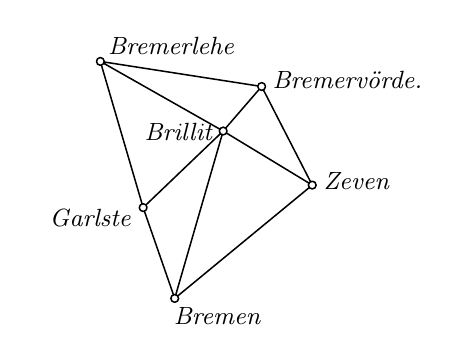
\begin{tikzpicture}[x=.0055cm,y=-.0055cm,line width=.55pt,line cap=round,line join=round,
 every node/.style={font=\small\itshape,inner sep=1pt}]
\path[use as bounding box] (0,0) rectangle (930,700);
\coordinate (Lehe) at (168,78); \coordinate (Voerde) at (541,136);
\coordinate (Brillit) at (452,239); \coordinate (Zeven) at (658,364);
\coordinate (Garlste) at (267,416); \coordinate (Bremen) at (340,626);
\draw (Lehe)--(Voerde)--(Zeven)--(Bremen)--(Garlste)--(Lehe)
 (Lehe)--(Brillit)--(Zeven) (Voerde)--(Brillit)--(Garlste) (Brillit)--(Bremen);
\foreach \v in {Lehe,Voerde,Brillit,Zeven,Garlste,Bremen}
 \draw[fill=white] (\v) circle[radius=1.4pt];
\node[anchor=south west] at (178,70) {Bremerlehe};
\node[anchor=south west] at (558,148) {Bremervörde.};
\node[anchor=east] at (434,240) {Brillit};
\node[anchor=west] at (676,354) {Zeven};
\node[anchor=east] at (246,439) {Garlste};
\node[anchor=north west] at (330,638) {Bremen};
\end{tikzpicture}
\end{center}
\noindent $2\frac12{}''$ sinkt. Aber auch dieser Rest kann gewiss nicht ganz den Mes-

% Printed 493; principal PDF 500; Google PDF 504.
\par\clearpage
\noindent\null\hfill{\small\textbf{MESSUNGSFEHLER.}}\hfill\makebox[0pt][r]{\fontsize{13}{16}\selectfont 493}\par\medskip
\noindent sungsfehlern zugeschrieben werden. Namentlich ist in Bremen der obige Fehler 1) durch das Vorwärts- und Rückwärtsmessen fast ganz beseitigt. Auch die Art des Anvisierens kann wenig Einfluss haben, da die Lichter bei der beträchtlichen Entfernung und der gewöhnlichen Unsichtbarkeit der Türme so gut wie frei erschienen.\par
\noindent .\ .\ .\ .\ .\ .
\begin{center}{\large\textsc{Gauss} an \textsc{Schumacher}.\quad Göttingen, 14. August 1825.}\end{center}
\par\noindent\hspace*{\parindent}.\ .\ .\ .\ .\ .\enspace Beträchtliche Abweichungen bei meinen Messungen haben mich diesen Sommer sehr geplagt. Ich bin jetzt zwar überzeugt, dass in flachen Gegenden starke Lateralrefraktionen auftreten können, wenn das Licht dicht über oder neben Gehölz vorbeistreicht, und dass sie in den zum Messen geeigneten Stunden stets in derselben Richtung wirken. Ebenso gewiss ist aber, dass andere Fehlerquellen hinzukamen, denen ich inzwischen ziemlich auf die Spur gekommen bin. Besonders den folgenden beiden.\quad 1) Das Anvisieren von Heliotroplicht \textls[120]{zwischen} den Fäden eignet sich, zumal bei schwachem Licht, nicht, wenn das Licht nicht frei liegt, sondern sich zum Beispiel außermittig in der Laterne eines Turms befindet, die selbst ziemlich gut sichtbar ist. Dadurch können konstante Fehler von mehr als $2''$ entstehen. Seit ich mich davon überzeugt habe, habe ich in solchen Fällen immer \textls[120]{auf} einem Faden anvisiert und dadurch die Abweichungen zum Teil erheblich vermindert.\quad 2) Der Theodolit gibt, wenn er so gebaut ist wie die unseren, eindeutig alle Winkel zu klein an. Der Durchschnittswert des Fehlers (der von der Größe des Winkels wenig abzuhängen scheint) lässt sich sehr genau bestimmen, mag aber mit fortschreitender Abnutzung des Instruments immer weiter zunehmen. In Brillit fand ich $0\overset{\prime\prime}{,}723$, wobei der wahrscheinliche Fehler unter $0\overset{\prime\prime}{,}1$ liegen dürfte. In Jever hatte ich nur etwa $0\overset{\prime\prime}{,}5$. Ich weiß noch nicht sicher, ob die Hauptquelle des Fehlers in der Klemmung des Limbuskreises (besonders in der Kugel), in der Hülse, die das untere Fernrohr trägt, oder in der Schraube liegt, die diese Hülse gegen den Fuß des Instruments hält. Letztere ist an meinem Instrument ziemlich abgenutzt. Für Versuche lasse ich jetzt die Klemmung des Limbuskreises unmittelbar am Fuß des Instruments anbringen, wobei ich das untere Fernrohr ganz entfernen werde. Ich halte es bei einer festen Aufstellung für unnütz und sogar für nachteilig, insofern seine Hülse als Zwischenstück zur Befestigung des

% Printed 494; principal PDF 501; Google PDF 505.
\par\clearpage
\noindent\makebox[0pt][l]{\fontsize{13}{16}\selectfont 494}\hfill{\small\textbf{BRIEFWECHSEL.}}\hfill\null\par\medskip
\noindent Limbuskreises am Fuß die Gefahr vervielfacht, dass sich der Limbuskreis bewegt, während man voraussetzt, dass er feststeht. Ich hätte sehr gerne einmal ausführlich mit Ihnen über diese Dinge gesprochen und meine Erfahrungen und Ansichten mit Ihren ausgetauscht.
\par\bigskip
\begin{center}{\large\textsc{Gauss} an \textsc{Bessel}.\quad Göttingen, 29. Oktober 1843.}\end{center}
\par\noindent\hspace*{\parindent}.\ .\ .\ .\ .\ .\enspace Es geht um eine Erfahrung, die mich oft geplagt hat, nämlich dass Theodolite nach der Konstruktion von \textsc{Reichenbach} dazu neigen, alle Winkel zu klein anzugeben. Vielleicht haben Sie ähnliche Erfahrungen gemacht, die ich gerne mit meinen austauschen würde.

\par\noindent\hspace*{\parindent}Bei meinen Winkelmessungen für die Gradmessung von 1821 bis 1823 und bei der anschließenden Erweiterung meiner Dreiecke 1824 und 1825 habe ich zwei verschiedene 12-zöllige Theodolite gebraucht (Nonien mit einer Ablesung auf $4''$, Vergrößerung etwa 35-fach). Den einen, den mir \textsc{Schumacher} geliehen hatte und der von \textsc{Reichenbach} selbst stammte, verwendete ich nur im Jahr 1821. Den anderen von \textsc{Ertel}, der dem ersten ganz gleicht und der Sternwarte gehört, verwendete ich von 1822 bis 1825. Beim ersten habe ich die Erscheinung überhaupt nicht bemerkt, beim anderen in den ersten drei Jahren und zu Beginn von 1825 ebenfalls nicht. Erst in der letzten Hälfte der Messungen bemerkte ich sie, zwar nur in geringem Ausmaß, aber so deutlich, dass daran kein Zweifel bestand. Eine Erklärung zumindest für die Hauptquelle liegt allerdings nahe. Der Kürze halber nenne ich die beiden Objekte $A$, $B$ und setze voraus, dass $B$ rechts von $A$ liegt und dass die erste Anvisierung immer $A$ und die zweite $B$ gilt. Nachdem man abgelesen und auf $A$ eingestellt hat, löst und bewegt man die Alhidade, um $B$ zu erreichen. Die Annahme, dass der Kreis selbst während dieser Bewegung \textls[120]{absolut} feststeht, ist allerdings unsicher. Besteht das geringste, für sich genommen nicht erkennbare Spiel, so wird die Drehung der Alhidade den Kreis ein wenig in derselben Richtung (von links nach rechts) mitdrehen. Die Differenz der Ablesungen gibt den Winkel also zu klein an. Auch bei noch so vielen Wiederholungen bleibt das Endergebnis immer zu klein.

\par\noindent\hspace*{\parindent}Als ich dies erkannt hatte, griff ich (in Jever) zu dem Mittel, zu einer Anzahl von Wiederholungen auf gewöhnliche Art

% Printed 495; principal PDF 502; Google PDF 506.
\par\clearpage
\noindent\null\hfill{\small\textbf{MESSUNGSFEHLER.}}\hfill\makebox[0pt][r]{\fontsize{13}{16}\selectfont 495}\par\medskip
\noindent stets ebenso viele hinzuzufügen, bei denen ich\ \raisebox{1.5ex}{\scriptsize.}\ die Alhidade von rechts nach links durch den Ergänzungswinkel zu $360^\circ$ bewegte. Dabei wurden nun alle Winkel immer größer als zuvor, und der Unterschied von durchschnittlich etwa 2 Bogensekunden schien überhaupt nicht oder wenigstens nicht merklich von der Größe der Winkel abzuhängen. Der Mittelwert der beiden Ergebnisse konnte also als wahrer Wert des Winkels gelten, und tatsächlich waren alle auf diese Weise gewonnenen Ergebnisse sowohl an dieser als auch an den übrigen Stationen vollkommen zufriedenstellend. Es schien also, dass dieser Theodolit in seinem damaligen Zustand alle auf gewöhnliche Art gemessenen Winkel um etwa eine Bogensekunde zu klein angab.

\par\noindent\hspace*{\parindent}Der ganze Kreis wurde von der ersten Ablesung bis zum ersten\linebreak
Anvisieren und später vom \begin{tabular}[c]{@{}c@{}}2.\\4.\\6.\end{tabular}\ usw. zum \begin{tabular}[c]{@{}c@{}}3.\\5.\\7.\end{tabular}\ usw. Anvisieren stets von\linebreak
rechts nach links bewegt (durch den Winkel $<180^\circ$). Es ist zumindest denkbar, dass sich auch hier eine stets in derselben Richtung wirkende Beeinflussung bemerkbar machen kann. Liegt das Spiel nämlich zum Teil in den Stellschrauben, Muttern oder Kugeln, so kann die Reibung des Alhidadenzapfens auf den ihn von unten stützenden Federn auch bei der Drehung des ganzen Kreises zu einer kleinen Verschiebung der Ablesung führen. Sie hätte dann gerade die umgekehrte Wirkung und würde die Winkel vergrößern. Ich habe jedoch vorausgesetzt, dass dieser Einfluss nicht wahrnehmbar ist. Es würde sehr viel Zeit kosten, darüber a posteriori Aufschluss zu erhalten. Ich brauche nicht daran zu erinnern, dass ich \textls[120]{stets} darauf geachtet habe, dass die Stellschrauben nicht zu leichtgängig waren.

\par\noindent\hspace*{\parindent}Zweifellos muss es irgendwo ein Spiel geben, aber es ist schwer festzustellen, \textls[120]{wo} es hauptsächlich auftritt. Ich habe später diesen Theodoliten ändern lassen, um das Spiel zu beseitigen, das bei der Drehung auftreten könnte, mit der man das Versicherungsfernrohr bewegt. Ich habe nämlich das bei fester Aufstellung ganz unnütze Versicherungsfernrohr ganz entfernt und den Arm, an dem sich die Kreisklemmung befindet, durch kräftige Winkelstücke unmittelbar mit dem Fuß verbinden lassen. Allerdings sind \textls[120]{nach} dieser Änderung zu wenige Messungen mit dem Instrument vorgenommen worden, um die Wirkung sicher beurteilen zu können.

% Printed 496; principal PDF 503; Google PDF 507.
\par\clearpage
\noindent\makebox[0pt][l]{\fontsize{13}{16}\selectfont 496}\hfill{\small\textbf{BRIEFWECHSEL.}}\hfill\null\par\medskip
\par\noindent\hspace*{\parindent}Bei den späteren Messungen von 1828 bis 1843 haben meine Offiziere drei andere Theodolite benutzt.
\par\noindent\hspace*{\parindent}1) \textsc{Hartmann} benutzte einen 8-zölligen Theodoliten von \textsc{Reichenbach}, den die Sternwarte schon seit 1813 besaß.
\par\noindent\hspace*{\parindent}2) \textsc{Müller} benutzte einen 12-zölligen Theodoliten von \textsc{Ertel}, der dem hannoverschen Generalstab gehörte (ich hatte ihn besorgt). Er war dem oben genannten ganz ähnlich, aber ohne Höhenkreis und Versicherungsfernrohr.
\par\noindent\hspace*{\parindent}3) Mein Sohn benutzte einen 8-zölligen Theodoliten von \textsc{Ertel}, ebenfalls ohne Höhenkreis und Versicherungsfernrohr, aber mit einem Fernrohr von genau derselben Stärke wie bei Nr. 2. Der Nonius erlaubt hier eine Ablesung auf $10''$.

\par\noindent\hspace*{\parindent}Bei Nr. 1 machte sich das Phänomen nicht bemerkbar. Das Instrument wurde übrigens nur ein paar Jahre benutzt und die Ergebnisse der Winkelmessungen fielen immer sehr gut aus. Das Fernrohr hat eine geringere optische Leistung, aber \textsc{Hartmann} hatte immer ein anderes, stärkeres Fernrohr eingesetzt, das ihm selbst gehörte. Ich erwähne diesen Umstand nur, um zu erklären, warum \textls[120]{dieser} Theodolit später nicht mehr benutzt wurde.

\par\noindent\hspace*{\parindent}Über Nr. 2 schreibe ich jetzt allein aus dem Gedächtnis und kann im Augenblick nicht genau sagen, \textls[120]{wann} das Phänomen erstmals auftrat. Wenn ich mich nicht irre, zeigte sich in den ersten Jahren keine besondere Spur davon. In den späteren Jahren war es aber unverkennbar und wenigstens doppelt so groß wie bei dem von mir benutzten Instrument. Jenes wurde oft zerlegt und gereinigt und, wenn ich mich recht erinnere, auch von \textsc{Hohnbaum} in Hannover mit neuen Stellschrauben versehen, ohne den Fehler zu beseitigen. Ich habe dem verstorbenen \textsc{Müller} stets das oben erwähnte Mittel dringend empfohlen, glaube aber nicht, dass er es immer konsequent angewandt hat.

\par\noindent\hspace*{\parindent}Mit Nr. 3 führte mein Sohn in den Jahren 1829, 1830, 1831, 1833 \textls[120]{sehr} ausgedehnte Messungen aus. Die Winkel (nebenbei bemerkt, an jeder Station werden in der Regel \textls[120]{alle} Kombinationen zwischen allen Hauptrichtungen gemessen, wie Sie auch aus den Arbeiten von \textsc{Gerling} ersehen können) stimmten immer zu meiner vollen Zufriedenheit, mindestens ebenso gut oder fast noch besser als die von \textsc{Müller} mit Nr. 2. Der Fehler zeigte sich jedenfalls nicht in erheblichem Ausmaß.

\par\noindent\hspace*{\parindent}Von 1834 an wurde dieser Theodolit etwa 5 oder 6 Jahre im magnetischen Observatorium benutzt und später zeitweise von \textsc{Goldschmidt} bei Winkelmessungen ge-

% Printed 497; principal PDF 504; Google PDF 508.
\par\clearpage
\noindent\null\hfill{\small\textbf{MESSUNGSFEHLER.}}\hfill\makebox[0pt][r]{\fontsize{13}{16}\selectfont 497}\par\medskip
\noindent braucht, die aber zu unbedeutend waren, als dass dabei der oben genannte Fehler hätte in Frage kommen können.

\par\noindent\hspace*{\parindent}Denselben Theodoliten Nr. 3 hat mein Sohn nun im vergangenen Sommer wieder für Hauptwinkel benutzt. An den Standpunkten, an denen die meisten Winkel gemessen wurden (auf Türmen in Hamburg und Stade), waren die Umstände in vielerlei Hinsicht äußerst ungünstig. Trotzdem trat das jetzige Vorhandensein jenes Minusfehlers, der wohl 3 bis $4''$ betrug, ganz eindeutig hervor. Der Theodolit war vor der Absendung hier gereinigt und überprüft worden, ohne dass irgendein Spiel bemerkt worden wäre. Mein Sohn fand jedoch das Ende der Stellschraube des Kreises ziemlich abgeschliffen. Die Beobachtungen der ersten Tage, an denen dies nicht beachtet worden war, wurden deshalb verworfen. Später wurde der Gebrauch dieses Teils der Schraube sorgfältig vermieden, und es ließ sich daran kein Spiel erkennen. Ich werde den Theodoliten nun wieder hierherkommen lassen und prüfen, ob ich durch Änderungen den Fehler oder wenigstens seine Wirkung beheben kann. Ich werde neue Klemmbacken anfertigen lassen. Ich bin noch unschlüssig, ob ich ganz neue Schrauben samt Zubehör anfertigen lasse, aus Sorge, vom Regen in die Traufe zu kommen. Da Sie selbst einen kleinen Theodoliten von \textsc{Meyerstein} erhalten haben, bitte ich Sie, gerade \textls[120]{diesen} Teil der Arbeit sehr sorgfältig zu prüfen und mir den Befund vertraulich mitzuteilen. Ich habe noch eine Idee für ein Mittel, das den Fehler (ein verborgenes Spiel) zwar nicht beseitigen, ihn aber hoffentlich unschädlich machen kann.

\par\noindent\hspace*{\parindent}Bekanntlich sind der Alhidadenzapfen und die Buchse dieses Zapfens, die ihrerseits den Zapfen des Limbuskreises bildet, von unten jeweils auf eigenen Federn abgestützt. Diese Federn will ich so ändern lassen, dass man ihre Spannung nach Belieben leicht und augenblicklich verstärken oder abschwächen kann. Die Spannungen sollen während der Messungen planmäßig gewechselt werden. Beim Drehen der Alhidade sind die Federn, auf denen ihr Zapfen ruht, stark gespannt, die Federn, die die Buchse stützen, fast gar nicht, und beim Drehen des ganzen Kreises ist es umgekehrt. \textsc{Meyerstein} glaubt, eine solche Änderung zweckmäßig einrichten zu können, und ich verspreche mir davon viel Erfolg. Nur schade,
\par\medskip\noindent\makebox[0pt][l]{\small IX.}\makebox[.86\linewidth][r]{63}\par
